\section{Introduction}

Le lancer de rayons (\textit{ray tracing}) constitue aujourd'hui une approche numérique largement utilisée dans des domaines scientifiques et industriels variés. Initialement popularisée par la synthèse d'images pour le rendu photoréaliste, cette méthode est désormais employée dans des applications aussi diverses que la simulation optique, le transport de particules ou le transfert radiatif. Malgré la diversité des phénomènes physiques considérés, ces applications reposent sur une problématique géométrique commune : déterminer efficacement les intersections entre un très grand nombre de rayons et une géométrie tridimensionnelle complexe.

Cette problématique a conduit au développement de bibliothèques logicielles spécialisées dans la navigation géométrique et l'accélération des calculs d'intersection. En physique des hautes énergies, le framework \textsc{ROOT} développé au CERN intègre ainsi le module de géométrie \texttt{TGeo}, conçu pour le suivi de trajectoires au sein de détecteurs complexes. Cette infrastructure géométrique a notamment servi de fondation au développement de \textsc{ROBAST}, une bibliothèque de lancer de rayons destinée à la simulation optique des télescopes Cherenkov \cite{Brun1997ROOT,Okumura2016}.

Parallèlement, les progrès réalisés dans le domaine du rendu graphique ont conduit au développement de bibliothèques dédiées à l'accélération des calculs d'intersection rayon--géométrie. Parmi celles-ci, \emb constitue aujourd'hui une référence pour les architectures CPU. Cette bibliothèque fournit des structures d'accélération hiérarchiques (\textit{Bounding Volume Hierarchies}, BVH) ainsi que des algorithmes de parcours fortement optimisés permettant de réduire significativement le coût des calculs géométriques \cite{Wald2014Embree}.

Les performances offertes par ces outils ont conduit à leur adoption dans plusieurs codes scientifiques. Par exemple, le modèle de transfert radiatif tridimensionnel \textsc{DART} s'appuie désormais sur Embree afin d'accélérer les tests d'intersection rayon--triangle lors des simulations de scènes urbaines et forestières complexes \cite{Qi2019HybridScene}. Cette convergence illustre le caractère transversal du lancer de rayons : indépendamment de la physique considérée, la recherche d'intersections constitue une brique algorithmique commune pouvant être mutualisée.

Le code de Monte Carlo Ray Tracing présenté dans ce chapitre s'inscrit dans cette démarche. Il s'appuie sur la bibliothèque \emb pour le traitement géométrique des trajectoires des rayons, tandis que les modèles physiques propres au transfert radiatif sont utilisés pour estimer les facteurs de vue entre les surfaces du domaine. 


\section{État du code à mon arrivée}

Le développement réalisé au cours de ce stage s'appuie sur une première maquette, issue d'un précédent stage. Cette maquette disposait déjà d'une chaîne fonctionnelle de lecture des maillages au format \ttt{.med} et de couplage géométrique avec la bibliothèque \emb, permettant de réaliser des calculs de facteurs de vue par lancer de rayons sur des géométries tridimensionnelles.

Ce socle logiciel présentait cependant plusieurs limitations. D'une part, sur le plan fonctionnel, le traitement de géométries quelconques n'était pas pris en charge. De même, la prise en compte de faces réflectives (miroirs), nécessaire pour modéliser certaines conditions aux limites de symétrie ou certains dispositifs expérimentaux, n'était pas implémentée. D'autre part, sur le plan de la fiabilité, les résultats produits par la maquette ne présentaient pas une précision satisfaisante par rapport aux facteurs de vue théoriques attendus, sans qu'un travail de vérification systématique n'ait été mené pour en identifier les causes. Cette absence de robustesse constituait un frein à l'utilisation du code en tant qu'outil de production, indépendamment même des fonctionnalités manquantes.

Ces constats — \textbf{fonctionnalités incomplètes} et \textbf{fiabilité insuffisante des résultats} — constituent le point de départ des travaux menés durant ce stage, dont l'objectif a été de consolider cette base existante et de l'étendre afin de répondre au cahier des charges détaillé ci-après.

\begin{figure}[H]
\begin{minipage}{0.52\textwidth}
\centering
\vspace{3.3em}
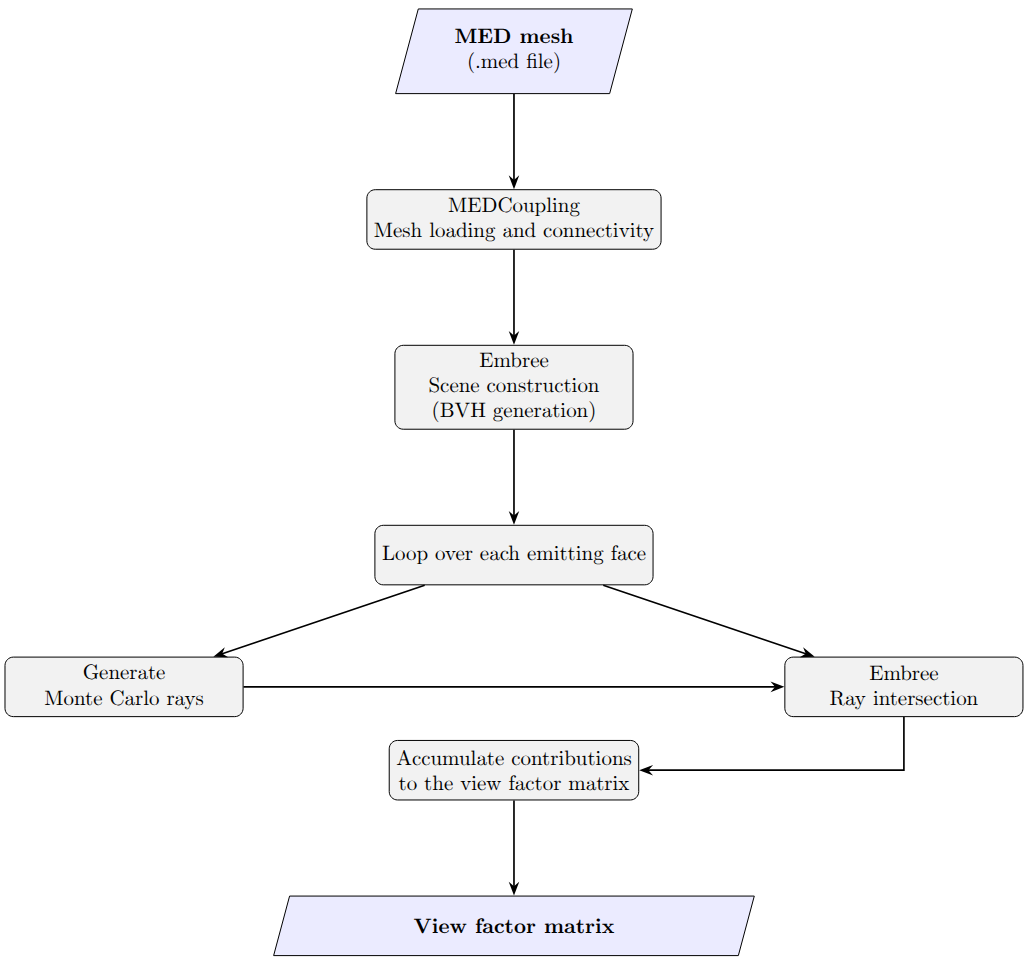
\includegraphics[width = 1\linewidth]{PICTURES/c2/E2T_diag.png}
\end{minipage}
\hfill
\begin{minipage}{0.5\textwidth}
\centering
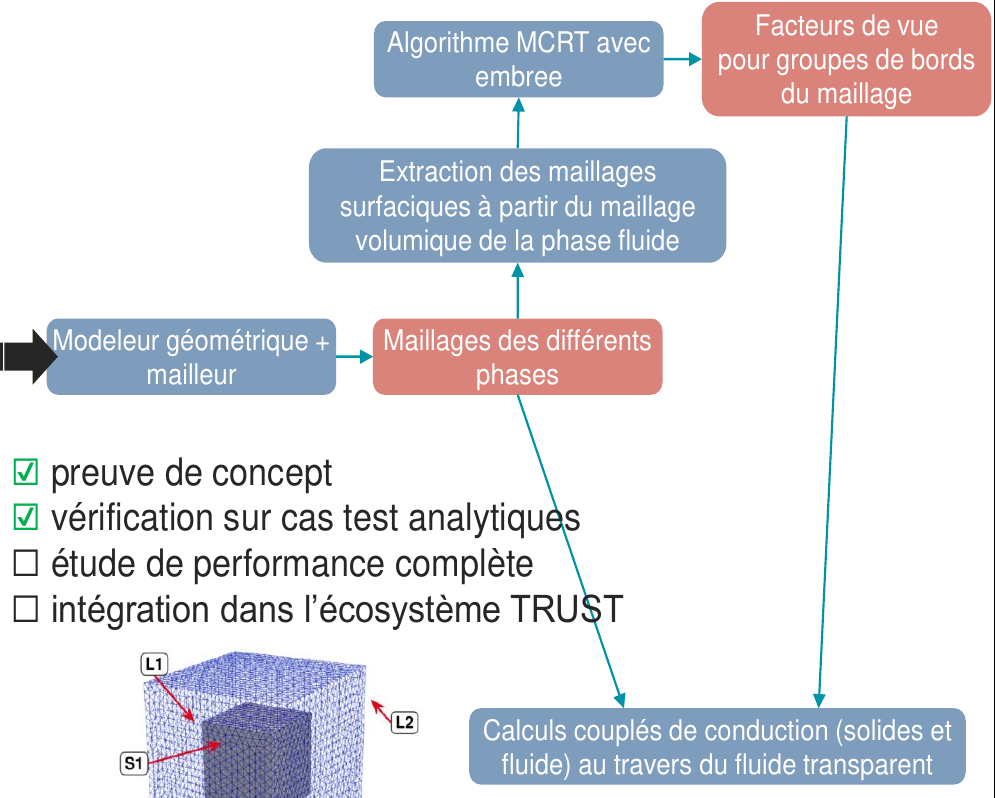
\includegraphics[width = 1\linewidth]{PICTURES/c2/chaine_calcul.png}
\vspace{0.3em}
\end{minipage}
\caption{Diagramme logique du code de lancer de rayons et de la chaîne de calcul}
\label{fig:diagramme}
\end{figure}

\section{Cahier des charges}

Le développement réalisé au cours de ce stage répond à un ensemble d'exigences fonctionnelles et techniques, définies en cohérence avec les besoins de la plateforme cible et avec les limitations identifiées dans la section précédente. Ces exigences sont résumées ci-après.

\begin{enumerate}
    \item \textbf{Exigences fonctionnelles}
    \begin{enumerate}
        \item L'outil doit permettre de simuler les échanges radiatifs entre les faces rayonnantes d'un fluide contenu dans une cavité, aussi bien pour des géométries bidimensionnelles que tridimensionnelles. Cette double compatibilité 2D/3D, absente de la maquette initiale, est nécessaire pour couvrir l'ensemble des cas d'usage rencontrés en aval de la chaîne de simulation, ces derniers pouvant relever indifféremment de l'une ou l'autre configuration selon la nature du problème traité.
        \item Le domaine de calcul est représenté par un maillage volumique tétraédrique, qui discrétise l'intérieur d'une cavité fermée correspondant au volume occupé par le fluide.
        \item La taille caractéristique du système traité doit être comprise entre le micromètre et le kilomètre, afin de couvrir l'ensemble des échelles rencontrées dans les cas d'usage visés.
    \end{enumerate}
    
    \item \textbf{Exigence de fiabilité}
    \begin{enumerate}
        \item Les facteurs de vue calculés doivent être fiables, et leur précision doit être quantifiée et maîtrisée.
        \item Cette exigence, motivée par le manque de robustesse constaté sur la maquette initiale, impose la mise en place d'une démarche de vérification systématique du code, comparant ses résultats à des solutions de référence pour des géométries variées.
    \end{enumerate}
    
    \item \textbf{Exigence d'interopérabilité}
    \begin{enumerate}
        \item Afin de s'intégrer nativement dans les cas de calcul existants, le code doit être capable de lire directement un maillage au format \ttt{.med}, format standard utilisé pour décrire la géométrie des domaines de calcul dans la chaîne de simulation visée.
        \item Cette contrainte exclut le recours à une représentation géométrique intermédiaire propre à l'outil radiatif, et impose que la géométrie utilisée pour le calcul des facteurs de vue soit rigoureusement celle du maillage fluide sur lequel repose la simulation couplée.
    \end{enumerate}
    
    \item \textbf{Exigence de performance}
    \begin{enumerate}
        \item Le code doit être performant, tant en termes de temps de calcul que d'utilisation des ressources disponibles.
        \item Cette exigence est dictée par la finalité du couplage visé : le calcul des facteurs de vue devant s'inscrire dans une simulation multiphysique plus large, il ne doit pas constituer un goulot d'étranglement pénalisant pour l'ensemble de la chaîne de calcul.
    \end{enumerate}
\end{enumerate}


\section{Avantages de la librairie \emb}

\subsection{Traitement vectoriel des rayons}

Le calcul des facteurs de vue nécessite le lancer d'un très grand nombre de rayons. La durée d'une simulation dépend donc directement du temps nécessaire au traitement de chaque rayon. Afin de réduire ce coût, le code s'appuie sur la bibliothèque \textsc{Embree}, développée par Intel et spécialisée dans le lancer de rayons haute performance.

L'une des principales optimisations proposées par cette bibliothèque consiste à traiter plusieurs rayons simultanément. Au lieu d'exécuter successivement les mêmes opérations sur chaque rayon, la librairie permet de regrouper les rayons par paquets et applique une même instruction à l'ensemble du groupe. Cette technique, appelée \emph{vectorisation}, permet d'exploiter les unités de calcul vectoriel présentes sur les processeurs modernes et de réduire le coût moyen de traitement d'un rayon.

La taille des paquets constitue un paramètre important de la bibliothèque. Une valeur trop faible n'exploite pas pleinement les capacités du processeur, tandis qu'une valeur plus élevée permet généralement d'améliorer les performances en augmentant le nombre de rayons traités simultanément. Une étude des ces performance est diponible en Annexe~\ref{annexe:perf_embree}.

\subsection{Accélération de la recherche d'intersections grâce aux BVH}

Dans un algorithme de lancer de rayons, l'étape la plus coûteuse consiste à déterminer le premier élément géométrique rencontré par chaque rayon. Une approche naïve consisterait à tester l'intersection avec tous les triangles du maillage, ce qui deviendrait rapidement prohibitif lorsque la géométrie comporte plusieurs milliers d'éléments.

Pour éviter ces tests inutiles, \textsc{Embree} construit automatiquement une \emph{Bounding Volume Hierarchy} (BVH). Cette structure organise les triangles du maillage dans une hiérarchie de boîtes englobantes (\emph{Axis-Aligned Bounding Boxes}, AABB), comme illustré Figure~\ref{fig:bvh}.

Lorsqu'un rayon est lancé, il est d'abord testé contre les boîtes englobantes. Si une boîte n'est pas traversée, tous les triangles qu'elle contient sont immédiatement éliminés. Les tests d'intersection précis ne sont finalement réalisés que sur les quelques triangles contenus dans les boîtes effectivement traversées par le rayon.

Cette organisation réduit considérablement le nombre de tests d'intersection et constitue l'une des principales raisons des performances élevées de \textsc{Embree}. Le coût de recherche d'une intersection devient ainsi beaucoup plus faible que dans une approche consistant à parcourir exhaustivement l'ensemble des triangles du maillage.

\begin{figure}[H]
    \centering
    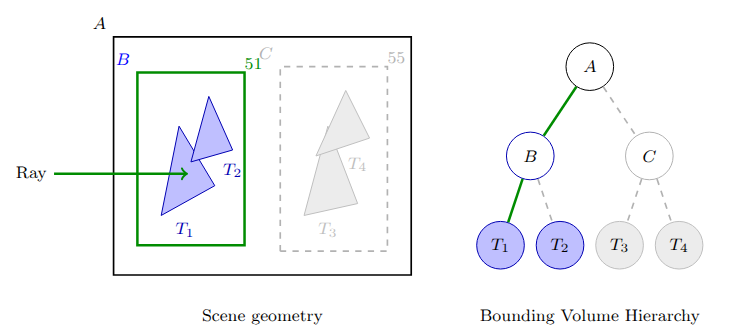
\includegraphics[width=0.8\linewidth]{PICTURES/c2/bvh.png}
    \caption{Principe d'une \emph{Bounding Volume Hierarchy} (BVH).}
    \label{fig:bvh}
\end{figure}




\section{Échantillonnage des rayons}

L'estimateur de Monte Carlo utilisé dans cette étude repose sur un échantillonnage direct des variables aléatoires intervenant dans la définition du facteur de vue. Les lois de probabilité sont choisies de manière à reproduire les distributions physiques de l'émission diffuse tout en conservant un poids unitaire pour chaque rayon. Cette stratégie correspond à l'approche dite de \textit{Monte Carlo analogue} (\textit{analog Monte Carlo}) couramment utilisée pour le calcul des facteurs de vue et des échanges radiatifs \cite{howell}.

L'émission d'un rayon est définie par le tirage de son point d'origine sur la surface émettrice, puis de sa direction dans l'hémisphère orienté par la normale locale.

\paragraph{Échantillonnage de la position}

Chaque surface est discrétisée par un ensemble de triangles. Afin d'obtenir une densité uniforme sur l'ensemble de la surface, le triangle $T_i$ est sélectionné avec une probabilité proportionnelle à son aire,

\begin{equation}
P(T_i)=\frac{A_i}{A_{\mathrm{tot}}},
\end{equation}

où $A_i$ est l'aire du triangle $T_i$ et $A_{\mathrm{tot}}$ l'aire totale de la surface.

Une fois le triangle sélectionné, le point d'émission est généré uniformément à l'intérieur de celui-ci au moyen de coordonnées barycentriques. La densité conditionnelle vaut alors

\begin{equation}
p(\mathbf{x}\mid T_i)=\frac{1}{A_i}.
\end{equation}

La densité de probabilité globale est donc

\begin{equation}
p(\mathbf{x})
=
P(T_i)\,
p(\mathbf{x}\mid T_i)
=
\frac{A_i}{A_{\mathrm{tot}}}
\frac{1}{A_i}
=
\frac{1}{A_{\mathrm{tot}}},
\end{equation}

ce qui garantit une distribution uniforme sur l'ensemble de la surface indépendamment de la discrétisation du maillage. L'utilisation des coordonnées barycentriques constitue une méthode classique pour réaliser cet échantillonnage uniforme sur des maillages triangulaires \cite{Pharr2018}.

\paragraph{cchantillonnage de la direction}

Sous l'hypothèse de surfaces diffuses grises, les rayons sont émis suivant une loi de Lambert. L'angle azimutal $\varphi$ est ainsi tiré uniformément dans l'intervalle $[0,2\pi]$,

\begin{equation}
\varphi \sim \mathcal{U}(0,2\pi),
\end{equation}

tandis que l'angle polaire $\theta$ suit une distribution cosinus dont la densité de probabilité par unité d'angle solide est

\begin{equation}
p(\omega)=\frac{\cos\theta}{\pi},
\qquad
0 \leq \theta \leq \frac{\pi}{2}.
\end{equation}

Cette distribution reproduit la loi d'émission lambertienne et constitue le choix naturel pour le calcul Monte Carlo des facteurs de vue, puisqu'elle est directement compatible avec les hypothèses physiques retenues dans cette étude. Son échantillonnage est réalisé selon la méthode classique par inversion de la fonction de répartition \cite{Pharr2018}.



\section{Compensation de l'approximation flottante sur l'origine du point}
\subsection{De manière systématique}
Afin d'éviter les auto-intersections lors de l'émission d'un nouveau rayon depuis un point d'impact, il est nécessaire de décaler légèrement son origine le long de la normale géométrique à la surface. Une approche couramment employée consiste à appliquer un décalage de longueur fixe $\varepsilon$. Cependant, cette méthode dépend de l'échelle géométrique du problème et ne garantit pas une élimination robuste des auto-intersections. Wächter et Binder \cite{Wachter2019} montrent qu'un décalage adaptatif obtenu en modifiant directement la représentation en virgule flottante des coordonnées du point d'intersection permet de produire un déplacement proportionnel à la précision numérique locale. Cette approche est ainsi pratiquement invariante vis-à-vis de l'échelle de la scène, ne nécessite aucun réglage de paramètre et limite efficacement les artefacts numériques tout en conservant un surcoût de calcul négligeable.

La Figure \ref{fig:offset} illustre le cas où la position calculée $p_{calc}$ est en "dehors" de la géométrie. La position théorique $p_{th}$ étant pile à l'interface. La position corrigée $p_{cor}$ est bien un décalage dans la direction de la normale de la surface.

Ces obversations ne sont pas présentées dans ce rapport. Mais l'approximation flottante des points d'intersection a notamment peut être mis à jour sur des géométries très simples. Les auto-inserections pouvant atteindre $75$~\% des rayons émis sur une face. Il est important de noter que cette correction est bien plus robuste que l'outils inhérent à la librairie \emb.

\subsection{Cas pathologique de tirage aux intersections de deux groupes}
De la même manière, un rayon peut être échantilloné sortant de la géométrie. Ce cas n'a lieu que lorsque le point est suffisamment proche d'une arrête d'un triangle, et que la frontière correspond à l'extérieur de la géométrie. La solution développée décale le rayon vers l'opposé la projection de la direction dans le plan d'émission (voir Figure \ref{fig:offset}). La probablité d'un tel tirage est extrêment faible. De plus, la correction est minime et ne change pas l'identité de la face récéptrice dans les conditions normales d'utilisation\footnote{La taille caratéristique du système doit être plus grande que le $\micro m$} du code.
\begin{figure}[H]
\centering

\begin{minipage}{0.4\textwidth}
\centering
\vspace{3.3em}
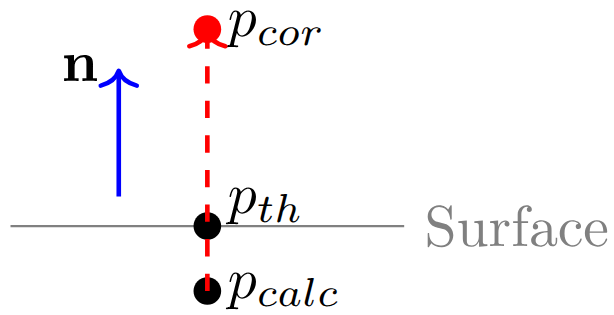
\includegraphics[width = 0.95\linewidth]{PICTURES/c2/offset_robust.png}

\small\textbf{(a) Décalage systématique}
\end{minipage}
\hfill
\begin{minipage}{0.5\textwidth}
\centering
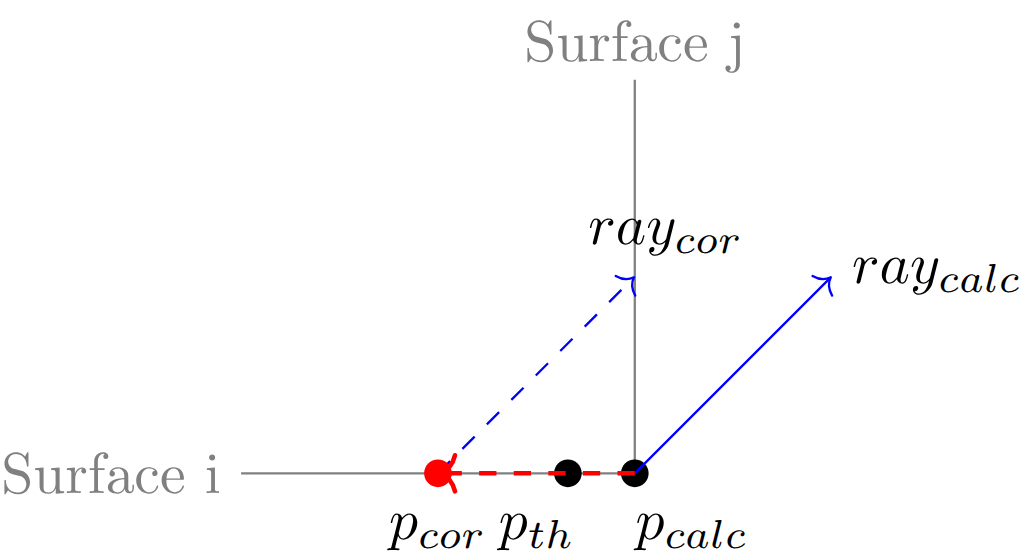
\includegraphics[width = 1\linewidth]{PICTURES/c2/offset_physic.png}

\vspace{0.3em}
\small\textbf{(b) Décalage des rayons sortants}
\end{minipage}

\caption{Illustration en 2D des décalages nécessaires pour corriger l'imprécision flottante de la position calculée .}
\label{fig:offset}

\end{figure}





